\documentclass{article}

\usepackage{graphicx}
\usepackage{indentfirst}
\usepackage[a4paper, total={6in, 8in}]{geometry}
\usepackage{hyperref}
\usepackage{fancyhdr}
\usepackage{xepersian}
\usepackage{fontspec}
\usepackage{url}
\settextfont[Scale=1.2,ExternalLocation=fonts/,BoldFont=B Nazanin Bold.ttf]{B Nazanin}
\setlatintextfont[Scale=1.2,ExternalLocation=fonts/,BoldFont=XB Zar.ttf]{Times New Roman}

\begin{document}


%title page%
\begin{titlepage}
	\begin{center}
		\vspace{0.2cm}
		
		
\includegraphics[width=0.4\textwidth]{sharif.png}\\
		\vspace{0.5cm}
		\textbf{ \Huge{فاز اول}}\\
		\vspace{0.25cm}
		\textbf{ \Large{پروژه مقدمه‌ای بر بیوانفورماتیک \\ دکتر علی  شریفی‌زارچی و دکتر سمیه کوهی}}
		\vspace{0.2cm}
		
		
		\large \textbf{دانشکده مهندسی کامپیوتر}\\\vspace{0.1cm}
		\large   دانشگاه صنعتی شریف\\\vspace{0.2cm}
		\large   ﻧﯿﻢ‌سال اول ۰۱-۰۲ \\\vspace{0.2cm}
		\large{\Large{امیرحسین باقری - 98105621}}\\
		\large{\Large{مهدی مستانی - 97100513}}\\
		\large{\Large{محمدرضا مفیضی - 98106059}}\\
	\end{center}
\end{titlepage}
%title page%

\newpage
\tableofcontents
\newpage
%pages header
\pagestyle{fancy}
\fancyhf{}
\fancyfoot{}
\setlength{\headheight}{59pt}
\cfoot{\thepage}
\lhead{فاز اول}
\rhead{
\includegraphics[width=0.1\textwidth]{sharif.png}\\
		دانشکده مهندسی کامپیوتر
}
\chead{پروژه مقدمه‌ای بر بیوانفورماتیک}
%pages header

\section{ریزآرایه چیست؟}
ریزآرایه \LTRfootnote{\lr{microarray}}، ابزاری آزمایشگاهی است که برای تشخیص بیان هزاران ژن به طور همزمان استفاده می‌شود. ریزآرایه‌های \lr{DNA} لام‌های میکروسکوپی هستند که با هزاران نقطه کوچک در موقعیت‌های مشخص چاپ می‌شوند و هر نقطه حاوی یک توالی \lr{DNA} یا ژن شناخته‌شده است.

 \subsection*{روش کار}
برای انجام تحلیل ریزآرایه، مولکول‌های \lr{mRNA} معمولاً از هر دو نمونه آزمایشی و نمونه مرجع جمع‌آوری می‌شوند. به عنوان مثال، نمونه مرجع را می‌توان از یک فرد سالم، و نمونه آزمایشی را می‌توان از یک فرد مبتلا به بیماری مانند سرطان جمع‌آوری کرد. سپس دو نمونه \lr{mRNA} به \lr{DNA} مکمل (\lr{cDNA}) تبدیل می‌شوند و هر نمونه با یک ترکیب فلورسنت \LTRfootnote{\lr{fluorescent}} با رنگ متفاوت برچسب‌گذاری می‌شود. مثلا، نمونه آزمایشی \lr{cDNA} ممکن است با رنگ فلورسنت قرمز برچسب‌گذاری شود، در حالی که \lr{cDNA} مرجع با رنگ فلورسنت سبز برچسب‌گذاری می‌شود.

 سپس دو نمونه با هم مخلوط شده و اجازه داده می‌شود تا به لام ریزآرایه متصل شوند. فرآیندی که در آن مولکول‌های \lr{cDNA} به ترکیب‌های \lr{DNA} روی لام متصل می‌شوند، هیبریداسیون \LTRfootnote{\lr{hybridization}} نامیده می‌شود.
پس از هیبریداسیون، ریزآرایه برای اندازه‌گیری میزان بیان هر ژن چاپ‌شده روی لام اسکن می‌شود. اگر بیان یک ژن خاص در نمونه آزمایشی بیشتر از نمونه مرجع باشد، نقطه مربوطه روی ریزآرایه قرمز به نظر می‌رسد.
از طرفی، اگر بیان در نمونه آزمایشی کمتر از نمونه مرجع باشد، آن نقطه سبز به نظر می‌رسد. در نهایت، اگر میزان بیان در دو نمونه یکسان باشد، نقطه زرد خواهد بود. داده‌های جمع‌آوری‌شده از طریق ریزآرایه‌ها را می‌توان برای ایجاد پروفایل‌های بیان ژن، که تغییرات همزمان در بیان بسیاری از ژن‌ها در پاسخ به یک بیماری یا درمان خاص را نشان می‌دهد، استفاده کرد. \cite{nature-microarray}
 
 \subsection*{فرمت داده‌‌های خروجی}
مجموعه داده‌های ریزآرایه معمولاً بسیار بزرگ هستند و فرمت داده‌های خروجی به صورت یک فایل خام (\lr{Raw Matrix}) در قالب یک متن \lr{tab-seperated} حاوی داده‌های بیش از یک سنجش ترکیبی (ترکیب‌ها در سطر‌ و نتایج آزمایش‌ها در ستون) است.
در تصویر \ref{fig:microarray} میزان بیان هر ژن به صورت \lr{heatmap} نمایش داده شده است.
\begin{figure}[h!]
	\centering
	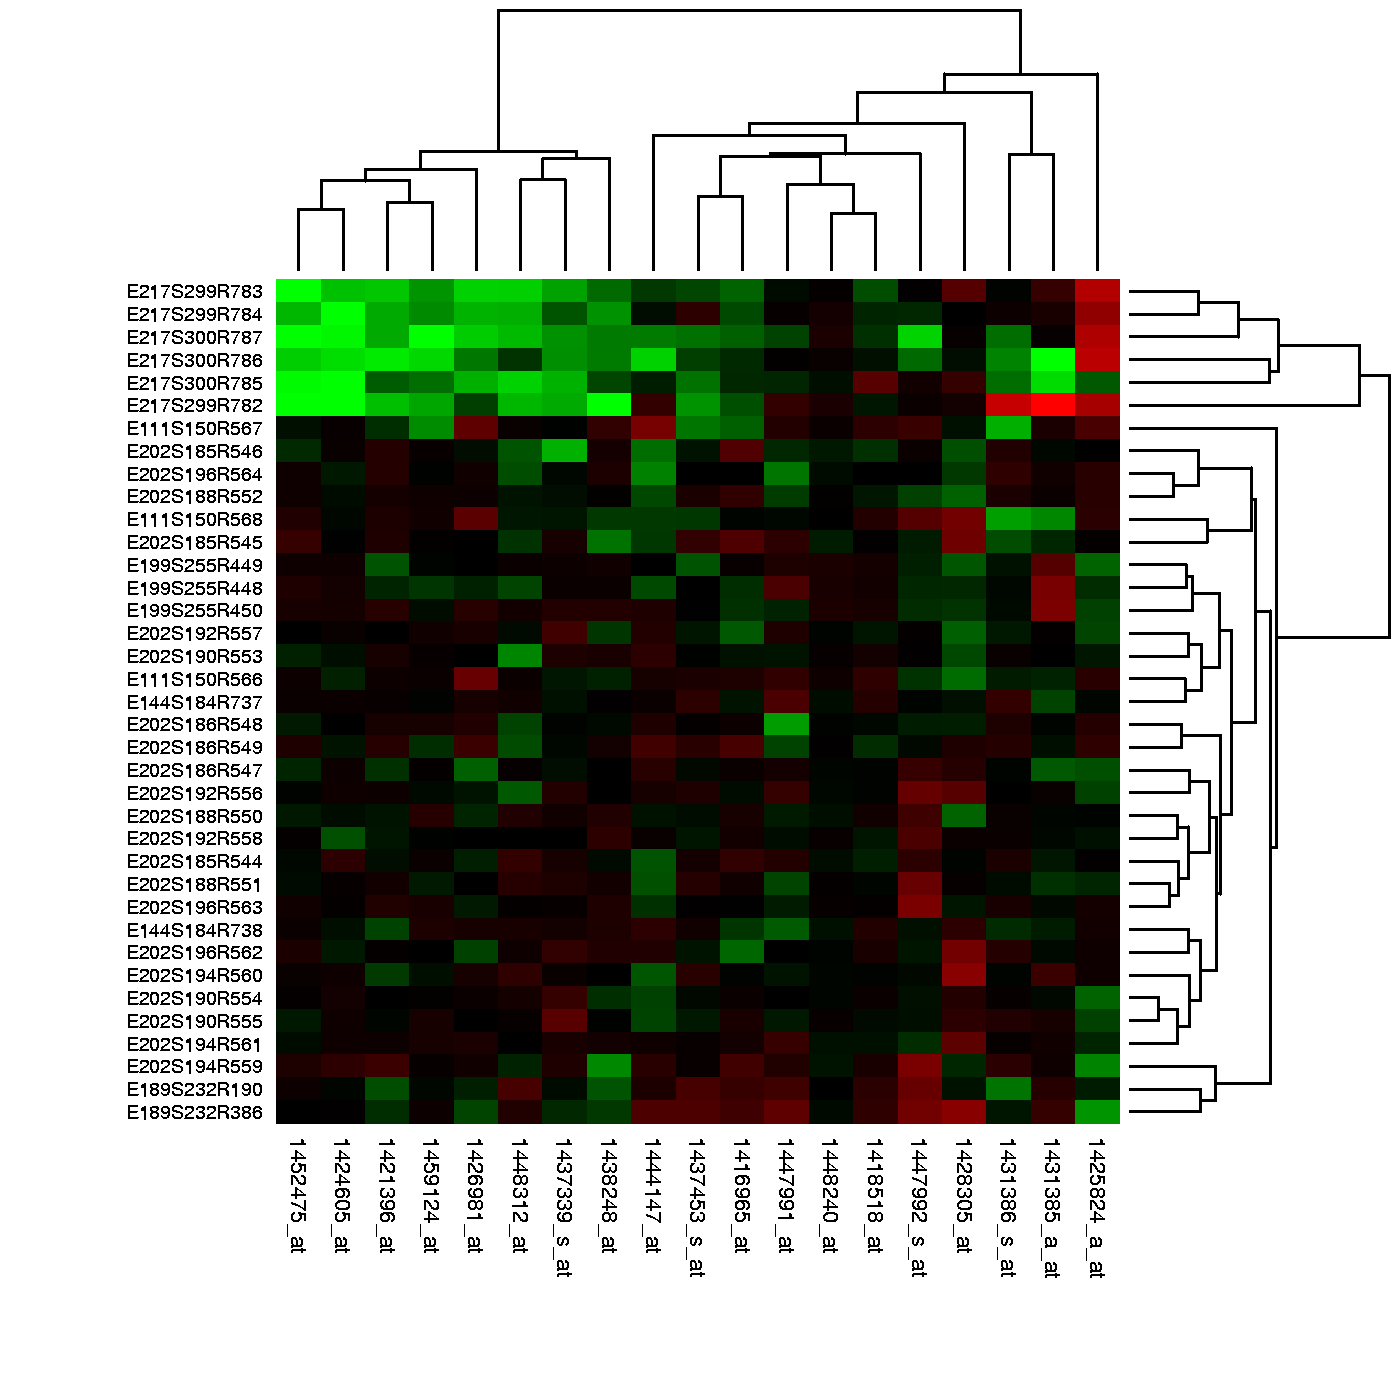
\includegraphics[width=0.5\columnwidth]{figs/microarray.png}
	\caption{میزان بیان ژن در ریزآرایه \cite{wiki-microarray}}
	\label{fig:microarray}
\end{figure}

همچنین داده‌های ریزآرایه در دیتاست با توجه به شکل \ref{fig:geo-data} قابل دسترسی خواهد بود.
\begin{figure}[h!]
 	\centering
 	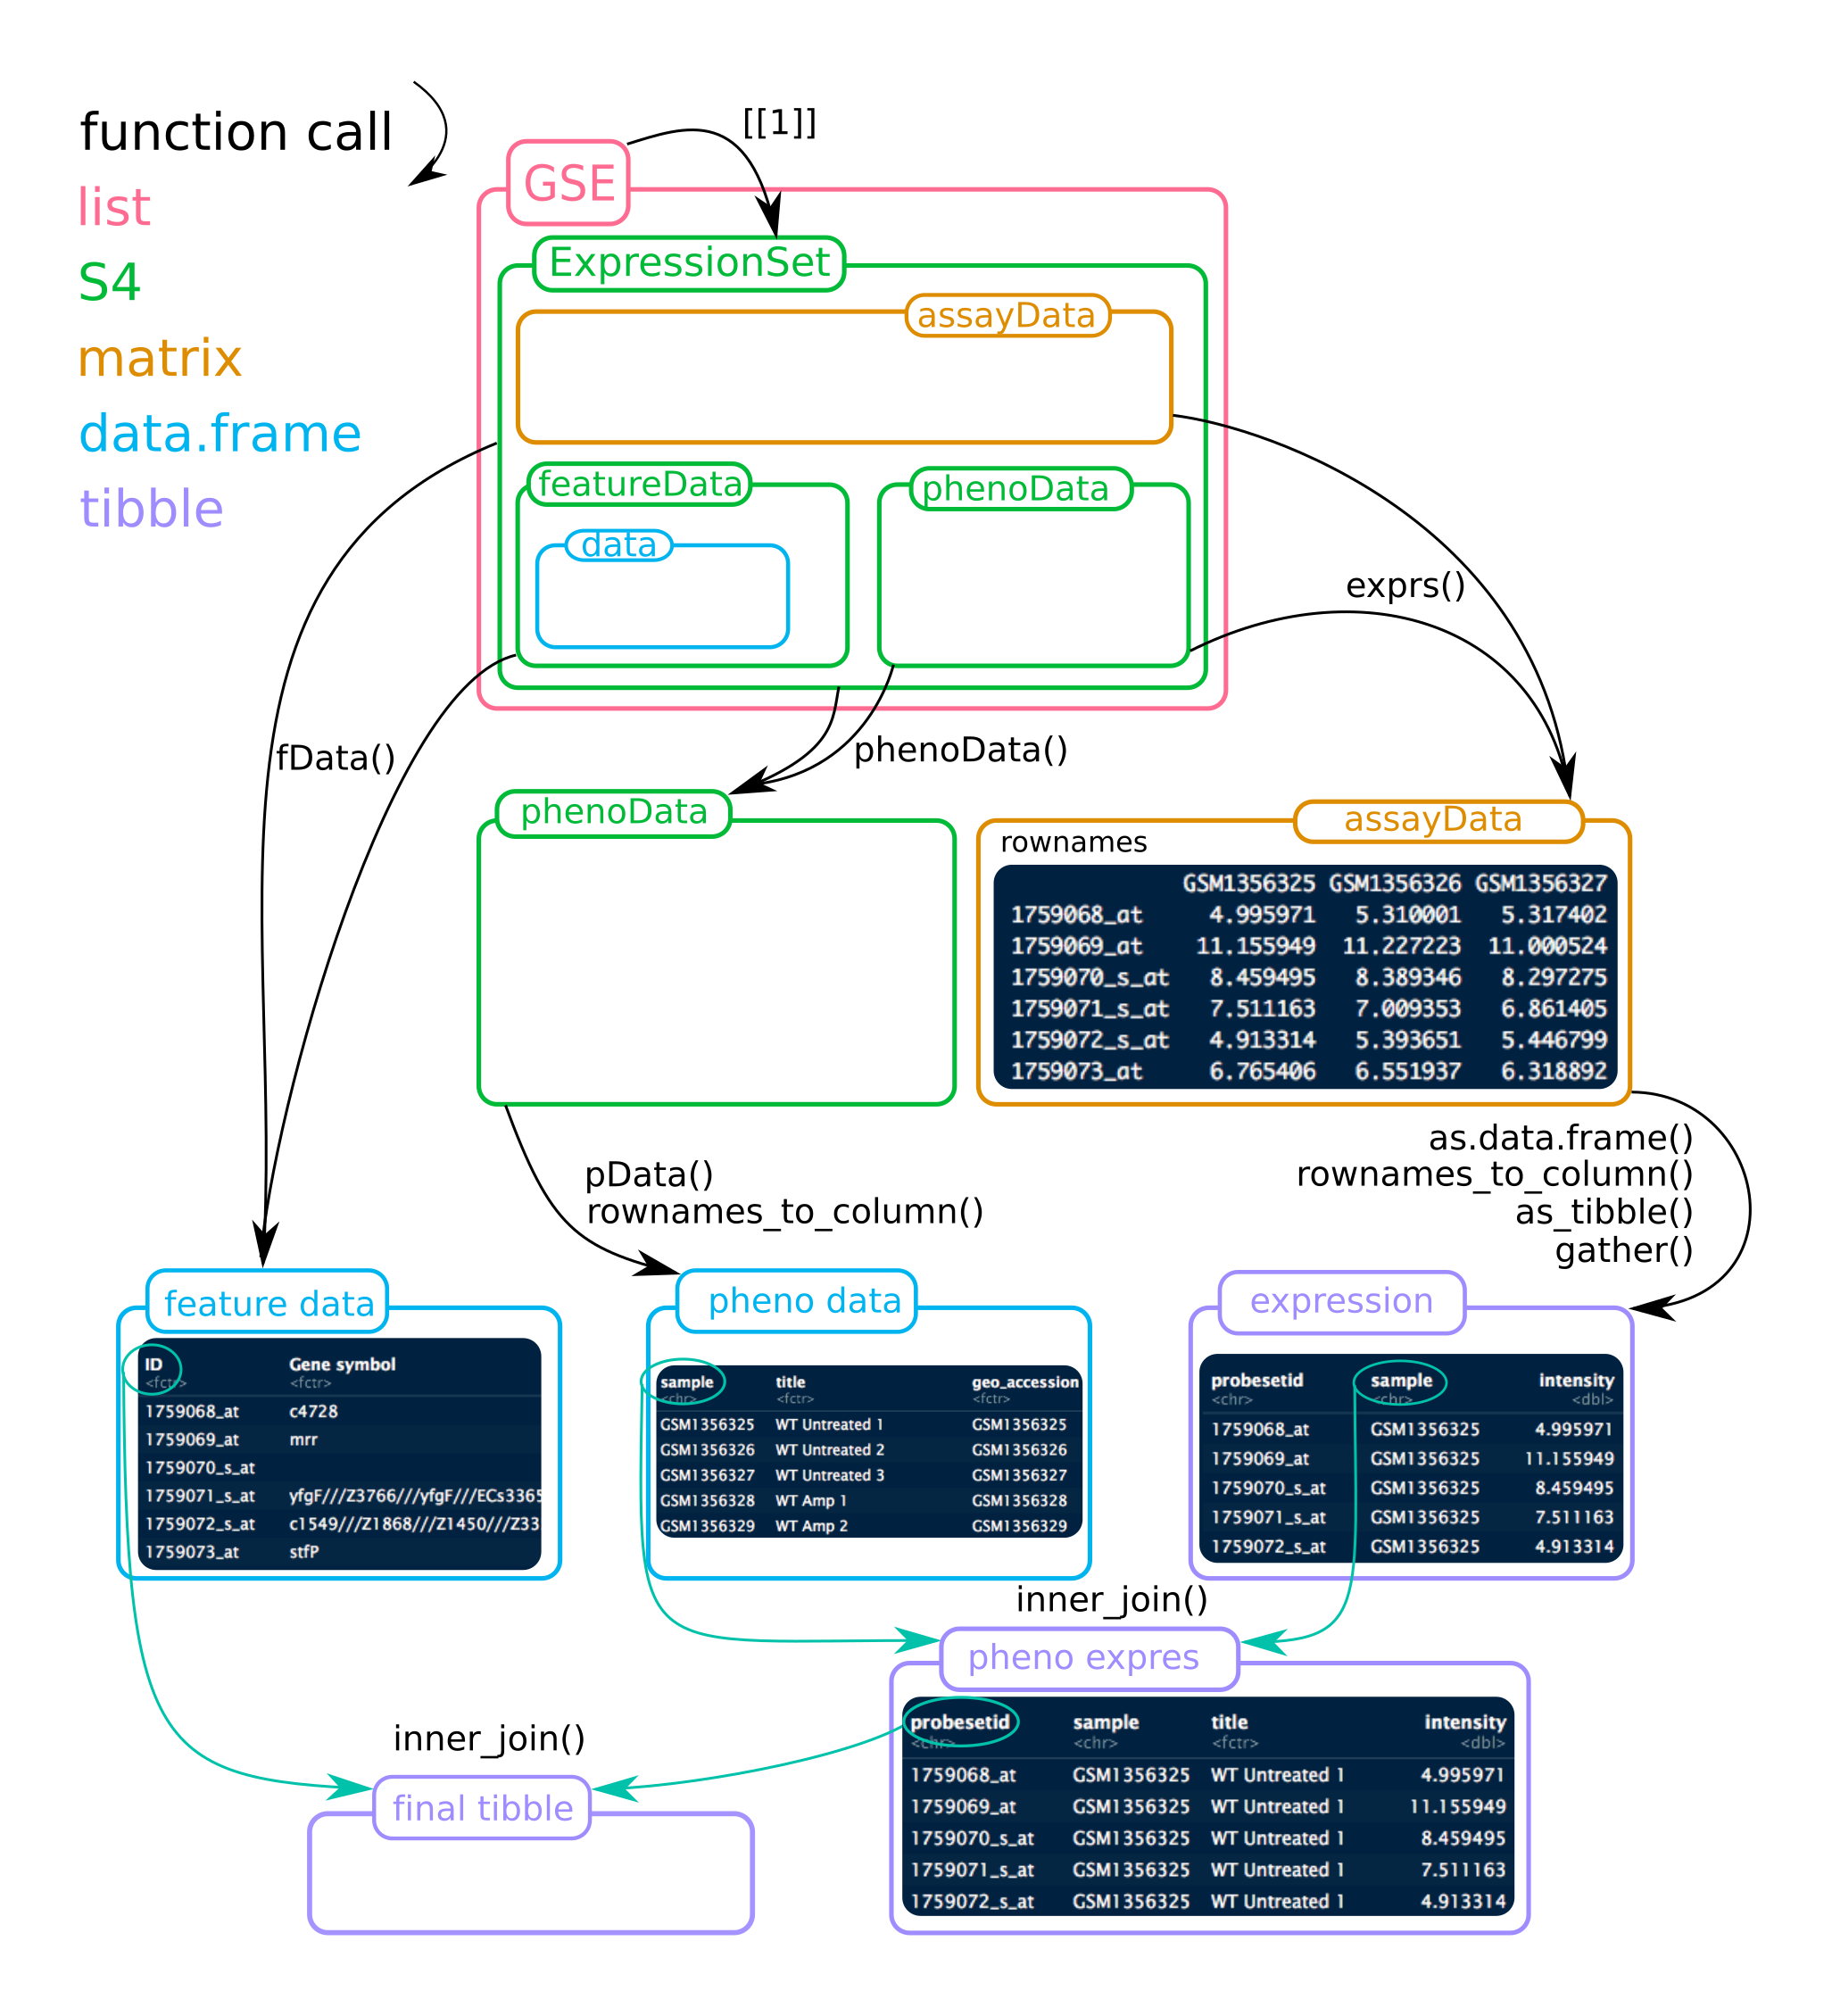
\includegraphics[width=0.8\columnwidth]{figs/geo-data.png}
 	\caption{ساختار داده‌ها در دیتاست \cite{geo-data}}
 	\label{fig:geo-data}
\end{figure}

\section{کیفیت داده‌ها}
در ابتدا بررسی می‌کنیم که بیشترین و کمترین مقدار داده‌ها در ماتریس بیان چقدر است. مشاهده می‌شود که بیشترین، عددی برابر با
$13.76154$
و کمترین برابر با
$1.611473$
است که نتیجه گیری این است که داده‌ها نرمال است(اگر که بیشترین مقدار عددی بیشتر از 100 بود از لگاریتم داده‌ها استفاده می‌کردیم تا نتیجه‌گیری‌های بهتری داشته باشیم). در ادامه نیز کد لازم در صورتی که داده‌ها نیاز به تبدیل به مقیاس لگاریتمی داشته باشیم، قرار داده‌شده‌است  تا صورت نیاز، این کار انجام شود (برای مثال اگر اختلاف ابتدا و انتهای بازه داده‌ها بیشتر از 50 باشد یا 1 درصد انتهای داده‌های عددی بیشتر از 100 باشد).
هم‌چنین داده‌های بدون مقدار و داده‌های تکراری را حذف می‌کنیم.
در انتها فقط بخشی از ستون‌های داده که اطلاعات بهتری به می‌دهند یعنی \lr{Accession} و \lr{SourceName} و \lr{Phenotype} را نگه ‌می‌داریم.

در ادامه به بررسی برخی از تحلیل‌های انجام‌شده روی داده‌‌ها می‌پردازیم.

برای بررسی‌های بیشتر در رابطه با آنالیز کیفیت داده‌ها، نمودار
\lr{Adjusted P-value}
را بررسی می‌کنیم. همان‌طور که در نمودار \ref{fig:adj-pv-dist} مشاهده می‌شود،  توزیع 
\lr{Adjusted P-value}
ها بدین صورت است که بخش قابل توجهی از آن‌ها در بازه $0$ تا $0.05$ قرار دارند که بیان‌گر این موضوع است که در بخش قابل از توجهی از داده‌ها تفاوت معنی‌داری وجود دارد  که یعنی نمونه‌های انتخاب شده این ویژگی را دارند که تفاوت‌های لازم را نمایش دهند. از طرفی نیز برای مقادیر بزرگتر‌ از 
$ 0.05$ 
نیز توزیع تقریبا یکنواختی را مشاهده می‌کنیم که این موضوع کیفیت خوب داده‌ها را تایید می‌کند؛ زیرا که بسیاری از ژن‌ها تفاوت بیان قابل توجهی در نمونه‌های مریض و سالم ندارند و در هر دو حالت بیان تقریبا یکسانی دارند.

\begin{figure}[h!]
	\centering
	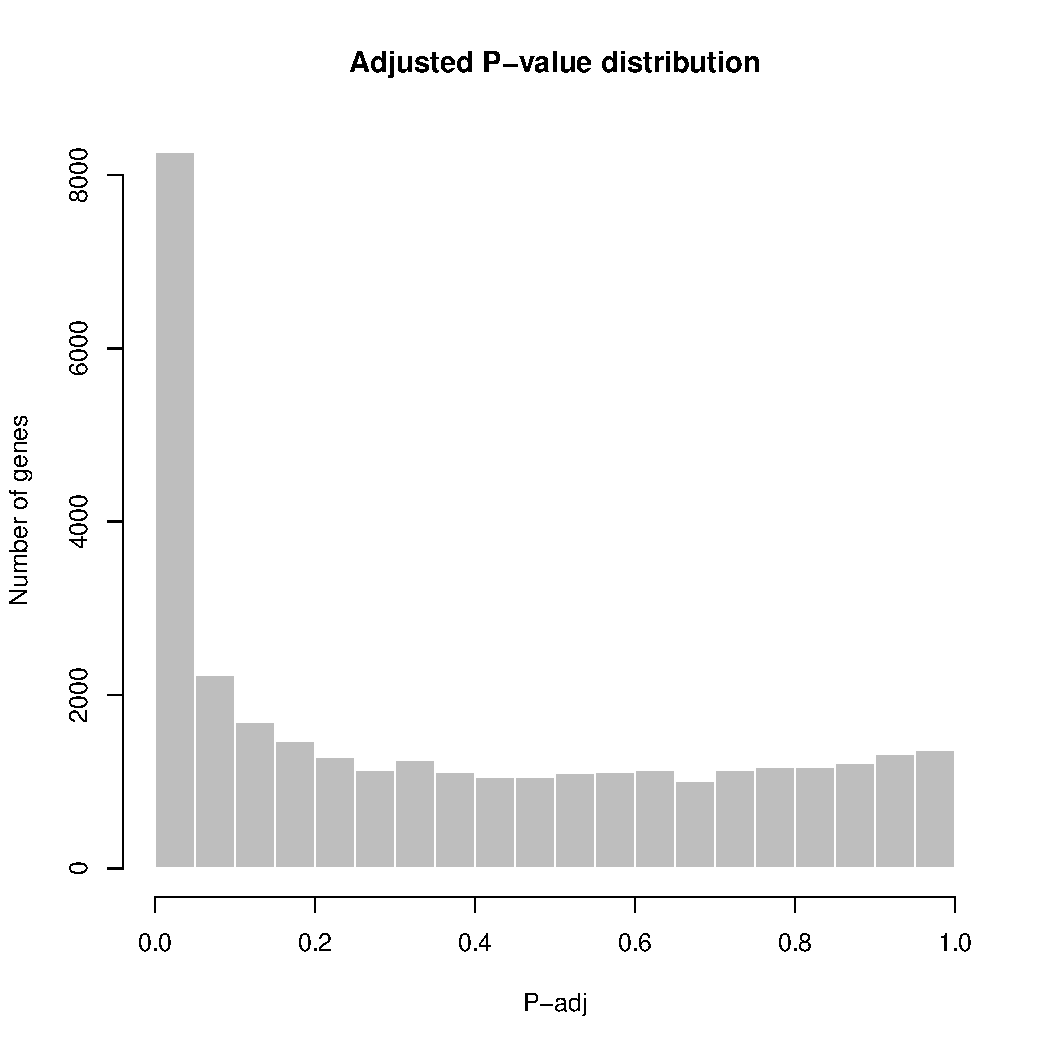
\includegraphics[width=0.5\columnwidth]{figs/adj-pv-dist.pdf}
	\caption{نمودار \lr{Adjusted P-value}}
	\label{fig:adj-pv-dist}
\end{figure}

سپس در نمودار \ref{fig:qq} چندک‌های \LTRfootnote{quantiles}  نمونه با چندک‌های تئوری که از توزیع
\lr{t-Student}
حاصل می‌شود را رسم می‌کنیم. مشاهده می‌شود که این نمودار تقریبا یک خط را توصیف می‌کند که یک حالت بسیار مناسب است که بیان‌گر این موضوع است که مقادیر مورد استفاده در نمونه از توزیع نظری پیش‌بینی شده تقریبا پیروی می‌کند.

\begin{figure}[h!]
	\centering
	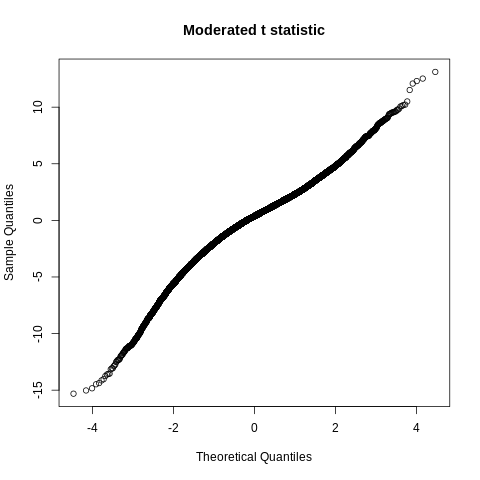
\includegraphics[width=0.5\columnwidth]{figs/qq.png}
	\caption{نمودار چندک‌های نمونه}
	\label{fig:qq}
\end{figure}

در مرحله بعد، نمودار آتشفشانی
\LTRfootnote{volcano plot} 
را بررسی می‌کنیم که این نمودار (شکل \ref{fig:volcano}) بدین صورت است که میزان اهمیت آماره (که در این آزمایش 
\lr{p-value}
است که البته برای نمایش بهتر آن از 
\lr{-log p-value}
استفاده می‌شود
)
در مقابل میزان تغییر دیتا (که در این قسمت نیز برای نمایش بهتر 
از 
\lr{lg fold change}
بهره می‌گیریم)
مورد بررسی قرار می‌گیرد.

\begin{figure}[h!]
	\centering
	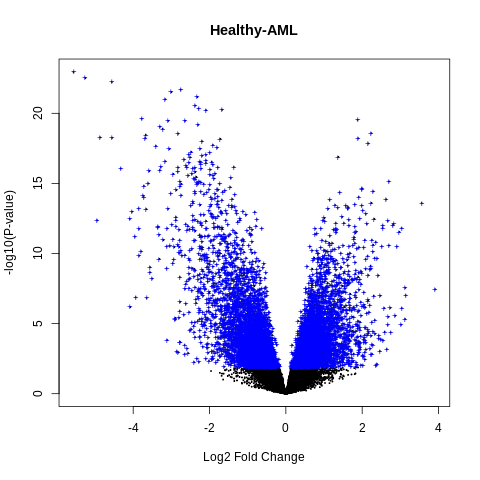
\includegraphics[width=0.5\columnwidth]{figs/volcano.png}
	\caption{نمودار آتشفشانی}
	\label{fig:volcano}
\end{figure}

در این نمودار، داده‌هایی که 
\lr{p-value}
آن‌ها مناسب است (کمتر 
$0.05$)
،
آبی شده‌اند و از طرفی ژن‌های آبی‌رنگ در سمت راست نمودار، میزان بیان آن‌ها در نمونه سالم بیشتر از بیمار است و ژن‌های آبی‌رنگ در سمت چپ نمودار، میزان بیان آن‌ها در نمونه بیمار بیشتر از سالم است و هر چه قدر به سمت راست و چپ نمودار حرکت کنیم، این تفاوت بسیار بیشتر و قابل توجه‌تر می‌شود . 
این نمودار بیان می‌کند که بخشی از ژن‌ها شرط 
\lr{p-value}
را برقرار نمی‌کنند و برخی از دیتا ها که این شرط را برقرار می‌کند، 
\lr{fold change}
آن‌ها چندان قابل توجه نیست  ولی تعدادی از داده‌ها که مقادیر 
\lr{p-value}
آن‌ها بسیار پایین است و نیز 
\lr{fold change}
آن‌ها مقادیر مثبت نسبتا زیاد دارند (نقاط بالا و سمت راست نمودار) و یا مقادیر منفی نسبتا زیاد دارند (نقاط بالا و سمت چپ نمودار) را می‌توان به‌طور ویژه بررسی نمود و در مجموع نمودار بیان می‌کند که کیفیت داده‌ها در مرحله قابل قبولی قرار دارد.

در قسمت بعدی نمودار اختلاف میانگین
\LTRfootnote{Mean Difference (MD) plot}
را بررسی می‌کنیم. این نمودار (شکل \ref{fig:md}) تا حدودی مشابه نمودار آتشفشانی عمل می‌کند با این تفاوت که 
$\log_2$
میانگین بیان ژن‌ها را در آن در نظر می‌گیریم و با 
\lr{lg fold change}
مقایسه می‌کنیم. در این نمودار  مقادیری  که 
\lr{p-value}
آن‌ها مناسب است (کمتر 
$0.05$
)
است و نیز 
$\log FC$
آن‌ها مثبت است را قرمز و آن‌هایی که منفی است را آبی کرده‌ایم.

\begin{figure}[h!]
	\centering
	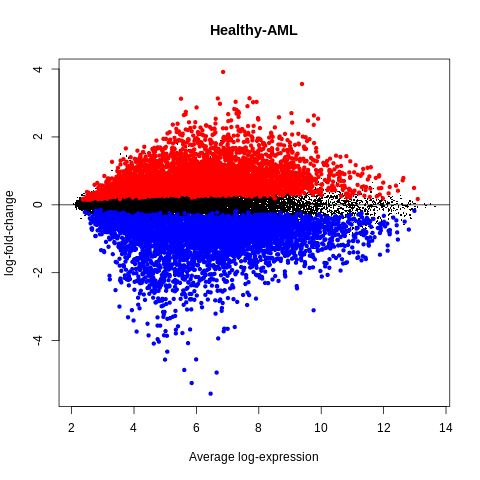
\includegraphics[width=0.5\columnwidth]{figs/md.png}
	\caption{نمودار اختلاف میانگین}
	\label{fig:md}
\end{figure}

در مرحله بعد، نمودار جعبه‌ای را مورد بررسی قرار می‌دهیم. نمودار حاصل (شکل \ref{fig:boxplot}) تقریبا نشان می‌دهد که میانه‌ی نمونه‌ها با یکدیگر برابر است که نشان‌گر این است که داده‌ها نرمال و قابل مقایسه هستند و از طرفی طول جعبه‌ها نیز این ویژگی را دارد . چارک‌ها و کمترین و بیشترین مقدار در هر یک از نمونه‌‌ها نیز تا حدودی با یکدیگر برابر است و از طرفی نیز بیشترین مقدار نمونه‌ها، عددی حداکثر 15 است که یعنی داده‌ها در مقیاس لگاریتمی می‌باشد و نیازی به تبدیل آن‌ها نیست.

\begin{figure}[h!]
	\centering
	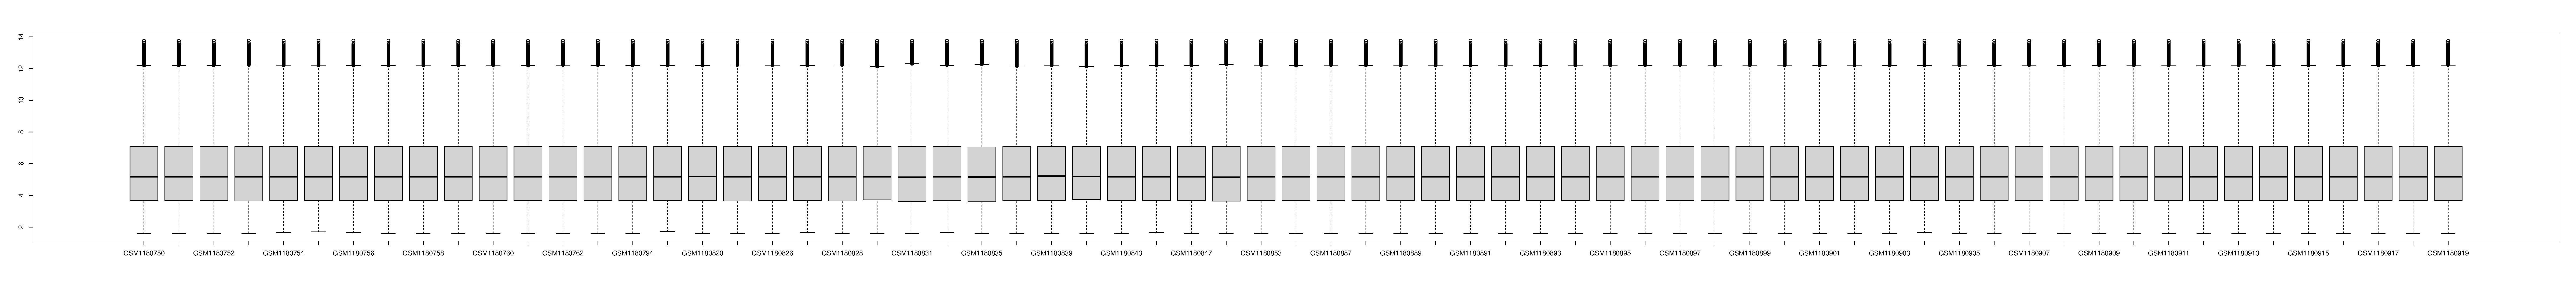
\includegraphics[width=0.8\columnwidth]{figs/boxplot.pdf}
	\caption{نمودار جعبه‌ای}
	\label{fig:boxplot}
\end{figure}

در بخش بعدی، نمودار توزیع چگالی بیان نمونه‌ها (شکل \ref{fig:exp-val-dist}) را بررسی می‌کنیم که در آن توزیع همه گروه‌های نمونه‌ها را با رنگ‌های متفاوتی در یک نمودار رسم می‌کنیم. مشاهده می‌کنیم که خم تمام گروه‌ها تقریبا بر یکدیگر منطبق است که بیان‌گر این است که نمونه‌ها نرمال و قابل مقایسه با هم هستند.

\begin{figure}[h!]
	\centering
	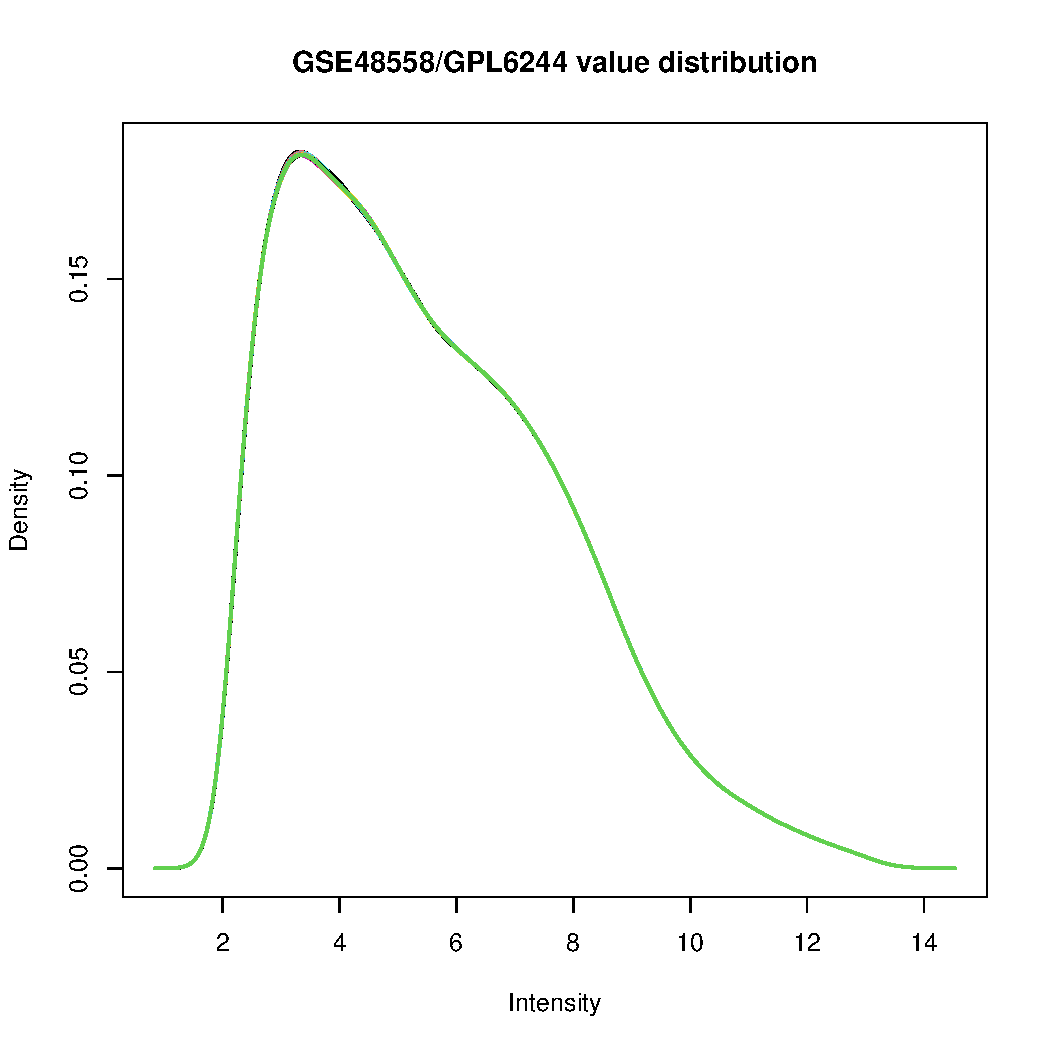
\includegraphics[width=0.5\columnwidth]{figs/exp-val-dist.pdf}
	\caption{نمودار توزیع چگالی بیان نمونه‌ها}
	\label{fig:exp-val-dist}
\end{figure}

همچنین نمودار \lr{Mean-Variance} (شکل \ref{fig:mean-var}) برای بررسی نسبت واریانس به میانگین میزان بیان ژن رسم شده که می‌تواند نشان دهد داده‌‌ها چقدر از هم پراکنده هستند.

\begin{figure}[h!]
	\centering
	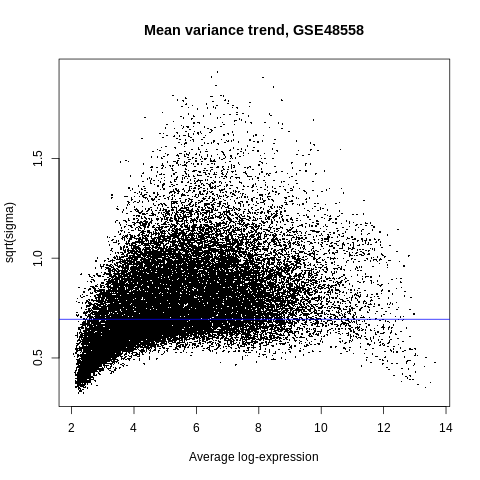
\includegraphics[width=0.5\columnwidth]{figs/mean-var.png}
	\caption{نمودار \lr{Mean-Variance}}
	\label{fig:mean-var}
\end{figure}

در انتها نیز از 
\lr{UMAP}
\LTRfootnote{Uniform Manifold Approximation and Projection}
استفاده می‌کنیم که یک روش کاهش بعد داده است که برای نحوه ارتباط داده‌ها با یکدیگر استفاده می‌شود. در نمودار \ref{fig:umap} مشخص است که نمونه‌های سالم به چند دسته تقسیم شده‌اند که البته در هر دسته نمونه‌ها بسیار شبیه به یکدیگرند (تقسیم آن‌ها به چند دسته نیز به این علت است که در نمونه‌های سالم نیز چند دسته‌ی متفاوت داشتیم) و از طرفی نمونه‌های بیمار نیز در یک دسته قرار دارند که موکد این است که نمونه‌ها از کیفیت مناسبی برخوردار هستند. البته اگر که توجه نماییم، برخی از نمونه‌های سالم در دسته‌ی بیمار قرار گرفته‌اند که در واقع بیان‌گر این است که این نمونه‌ها شباهت زیادی به نمونه‌های بیمار دارند که این نکته می‌تواند یکی از روش‌های یافتن نمونه‌های شبیه به بیمار در قسمت 4‌ام باشد.

\begin{figure}[h!]
	\centering
	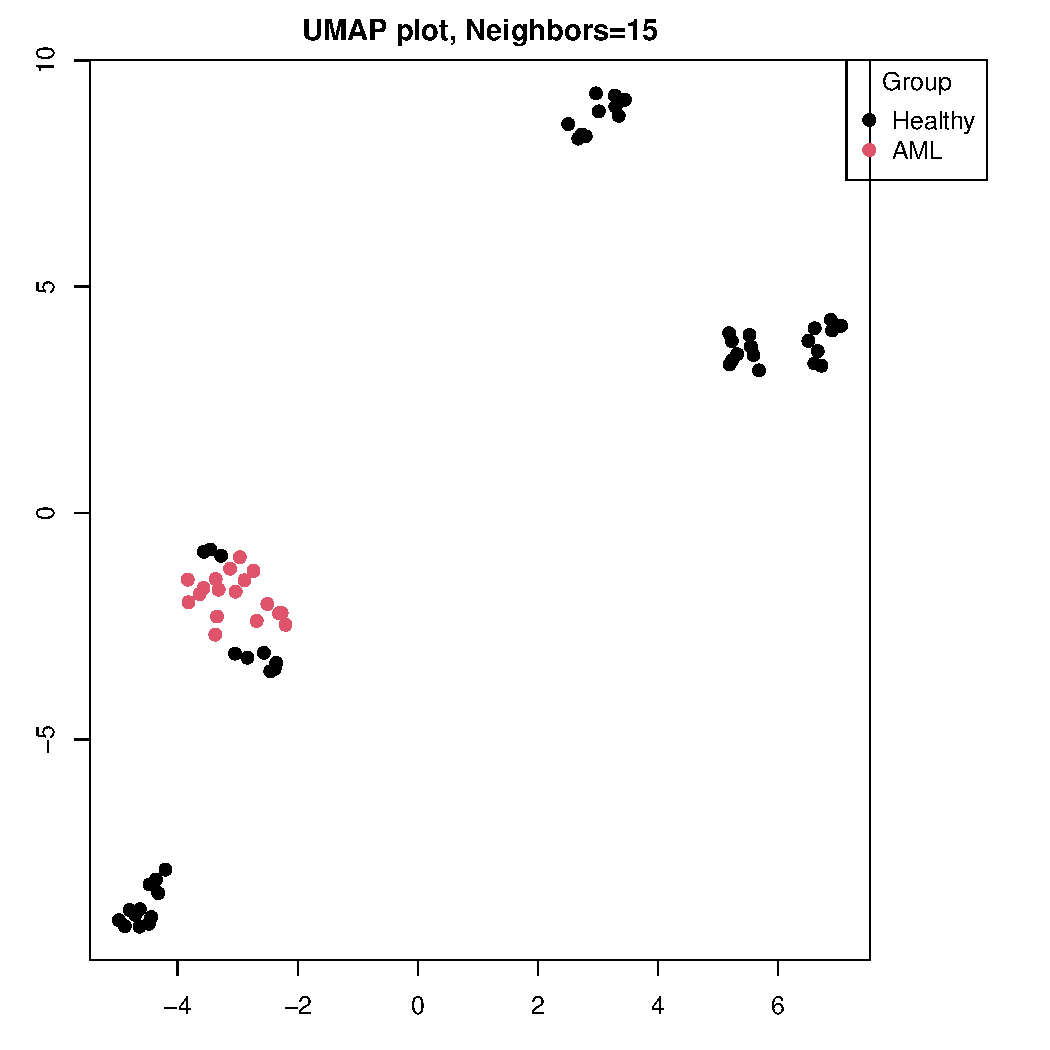
\includegraphics[width=0.5\columnwidth]{figs/umap.pdf}
	\caption{نمودار \lr{UMAP}}
	\label{fig:umap}
\end{figure}

\section{کاهش ابعاد داده‌‌ها}
\subsection{دلیل کاهش بعد داده‌ها}
کاهش ابعاد یک بعد کلیدی در مطالعات بایواینفورماتیک است. که به ما قابلیت نمایش دیتا های پیچیده و همچنین امکان بررسی آماری آنها را می‌دهد.
مطابق آنچه در درس دکتر شریفی گفته شد این کار برای ۲ مهم صورت می‌گیرد. زمانی که نتایج یک آزمایش در اختیار ما قرار می‌گیرد و ما می‌خواهیم یک مساله را بررسی کنیم. ممکن است که اشتباهی در فرایند جمع آوری داده رخ داده باشد ممکن است یک باکتری در محیط رشد کرده باشد و بناکردن نتایج تحقیقات بر روی یک داده ناصحیح ممکن است نتایج زیان باری داشته باشد بنابراین باید مطمعن شیم که داده های ما صحت دارند. برای این کار از کاهش بعد کمک می‌گیریم تا مطمعن شیم به طور مثال که آیا واقعا رابطه ای بین مساله و داده ها وجود ندارد یا اینکه داده ها صحت دارند و می‌توان کار را ادامه داد.


داده های بایوانفرماتیک عموما از پیچیدگی زیادی برخورداند بدین صورت که اکثر آنها تعداد نمونه ها از تعداد ویژگی ها بیشتر است  با کاهش بعد داده ها می توان داده ها را به متغیر های جدیدی تقلیل داد به طوری که تفاوت داده ها (تفاوت می تواند با متریک های متفاوتی اندازه گیری شود) حفظ شود.
تا بتوان داده هارا بررسی کرد.
\subsection{\lr{PCA}}
یک کاهش بعد خطی است که در نهایت داده هارا در یک ماتریس دوران ضرب می‌شود.
این کاهش بعد سعی می‌کند که در عین کاهش بعد بیشترین واریانس را حفظ کند. به دلیل اینکه به این پروژه مربوط نیست وارد توضیحات ریاضی آن نمی‌شویم و به همین توضیح بسنده می‌کنیم. 


\begin{figure}[!h]
	\centering
	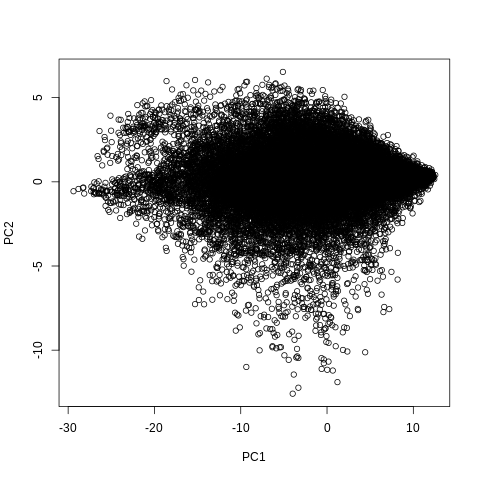
\includegraphics[width=0.5\columnwidth]{figs/pca2.png}
	\caption{میزان بیان هر ژن پس از کاهش بعد}
	\label{fig:pca2}
\end{figure}
ابتدا داده هایی که \lr{scale} نشده اند را بررسی می‌کنیم.
همانطور که می‌بینید در این داده ها به دلیل اینکه اختلاف بیان ژن ها مورد بررسی نیست و خود ژن ها مورد بررسی هستند. در نمودار آن داده ها بیان ژن ها به صورت بیضوی است به معنای آنکه بیان بعضی ژن ها زیاد و بیان بعضی کم است و این چیزی نیست که ما دنبال آن می‌گردیم.
(\ref{fig:pca2})

\begin{figure}[h!]
	\centering
	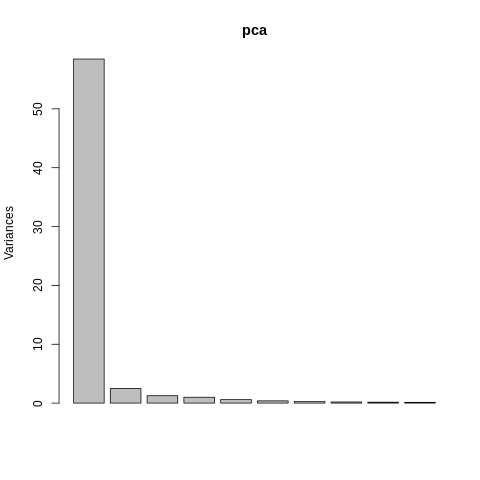
\includegraphics[width=0.5\columnwidth]{figs/pca3.png}
	\caption{واریانس هر بعد}
	\label{fig:pca3}
\end{figure}
همچنین در این حالت میزان واریانسی که در هر \lr{component}
وجود دارد میزان زیادی از آنها در بعد اول جمع شده( که همین عامل بیضوی شدن شکل شده است.) (شکل \ref{fig:pca3}
)
حال داده ها را که در ماتریس چرخش ضرب شده اند. در شکل \ref{fig:pca4} مشاهده می‌کنید که جدایی پذیری کمی دارند.

\begin{figure}[h!]
	\centering
	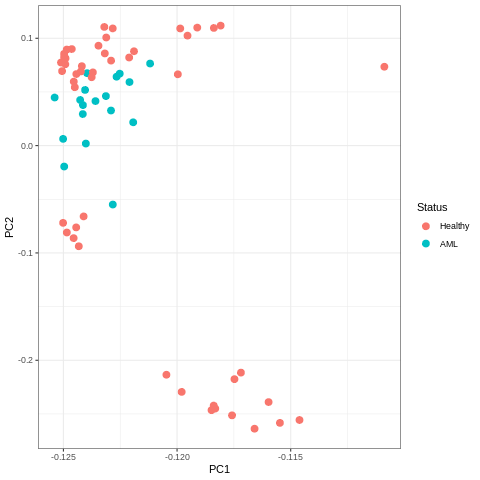
\includegraphics[width=0.5\columnwidth]{figs/pca4.png}
	\caption{داده های کاهش بعد یافته}
	\label{fig:pca4}
\end{figure}

حال داده های را \lr{scale} می‌کنیم بدان معنا که  میانگین هر سطور را از هر می‌کاهیم. بدین شکل تفاوت بیان ژن ها مشخص می‌شود.

همانطور که مشاهده می‌کنید واریانس موجود در هر \lr{component} اکنون قابل مقایسه شده است.
همچنین ژن ها در ۲ بعد از حالت بیضوی در آمده اند.
\ref{fig:pca5}
\begin{figure}[h!]
	\centering
	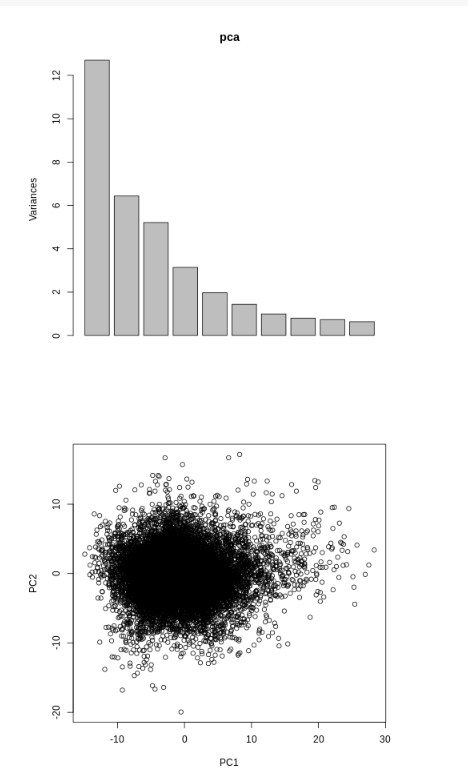
\includegraphics[width=0.5\columnwidth]{figs/pca5.png}
	\caption{ نتایج داده های اسکیل شده}
	\label{fig:pca5}
\end{figure}

حال کاهش بعد یافته داده هارا پس از اعمال اسکیل بر روی آنان در شکل \ref{fig:pca6}
مشاهده می‌کنید.
هماطور که مشاهده می‌شود در این حالت کاهش بعد بهتر عمل کرده و جدایی پذیری بیشتری بین گونه ها توانسته تشخیص دهد.
\begin{figure}[h!]
	\centering
	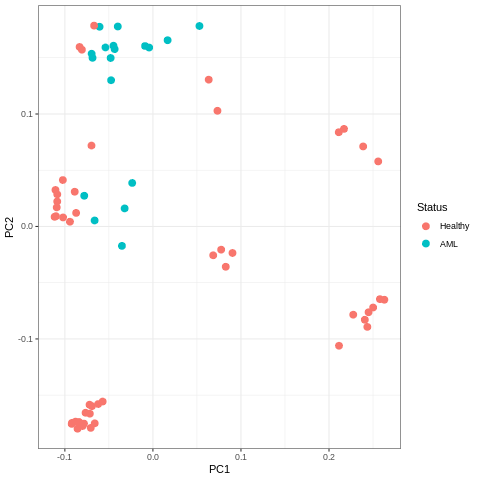
\includegraphics[width=0.5\columnwidth]{figs/pca6.png}
	\caption{ کاهش بعد یافته داده های اسکیل شده}
	\label{fig:pca6}
\end{figure}
\subsection{\lr{TSNE}}
\lr{(t-distributed Stochastic Neighbor Embedding)}
یک روش غیر خطی و احتمالاتی است که در سال ۲۰۰۸ معرفی گشته است.
این روش قادر است که داده هارا به طوری کاهش بعد دهد که جدایی پذیری آنان بسیار  عالی شود.
به عنوان مثال فرض کنید که داده ها بر روی یک خم (\lr{manifold})
قرار دارند. روش \lr{pca}
قادر به کاهش بعد آنان به صورتی که داده ها جدا سازی خوبی شده باشند ندارد اما \lr{TSNE}
می‌تواند این کار را انجام دهد.

به عنوان مثال داده های زیر در یک فضای ۳ بعدی بر روی ۲ خم قرار دارند. (شکل \ref{fig:tsne})

\begin{figure}[h!]
	\centering
	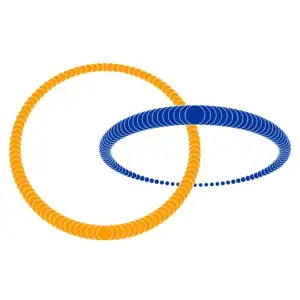
\includegraphics[width=0.4\columnwidth]{figs/tsne.png}
	\caption{داده ها در فضای ۳ بعدی}
	\label{fig:tsne}
\end{figure}


\begin{figure}[h!]
	\centering
	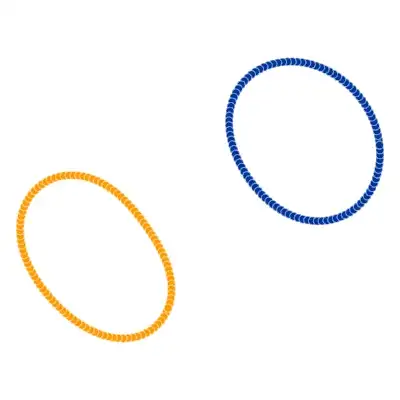
\includegraphics[width=0.4\columnwidth]{figs/tsne1.png}
	\caption{ کاهش بعد یافته آنان در فضای ۲ بعدی به کمک \lr{tsne}}
	\label{fig:tsne1}
\end{figure}

که کاهش شکل یافته آنان در فضای ۲ بعدی با استفاده از \lr{tsne}
به صورت شکل \ref{fig:tsne1} در می‌آید.

این الگوریتم یک معیار \lr{perplexity} نیز دارد که به معنای زیر است.
این مقدار برابر ۲ به توان آنتروپی شنون است. در واقع این متغیر برابر تعداد همسایه های موثر در الگوریتم است. در واقع می‌توان آن را به نوعی به تعداد همسایه های نزدیک در خم فضا ارجاع داد.
هر چه دیتا پر چگال تر باشد اندازه این متغیر باید بیشتر باشد تا به نتایج بهتری دست یابیم.
درواقع این معیار متناسب با اندازه دیتا ست خواهد شد.

در این بخش 
حال به کاهش بعد داده های اصلی می‌پردازیم.
در شکل \ref{fig:tsnep} مشاهده می‌کنید که مقدار ۵ از همه بهتر عمل می‌کند.
\begin{figure}[h]
	\centering
        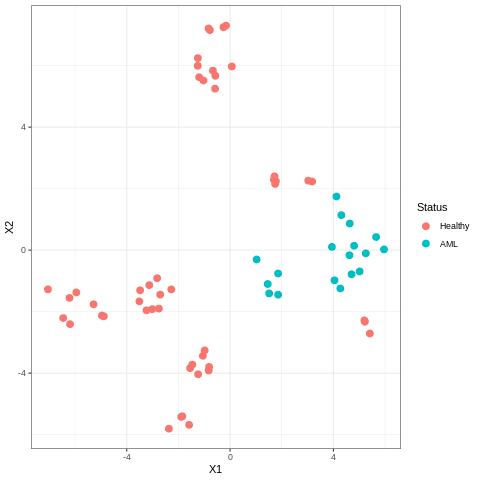
\includegraphics[width=.5\textwidth]{figs/tsnep20.png}\hfill
        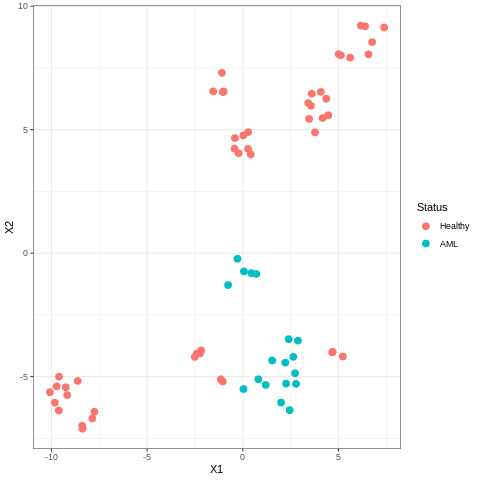
\includegraphics[width=.5\textwidth]{figs/tsnep15.png}\hfill
        \\[\smallskipamount]
        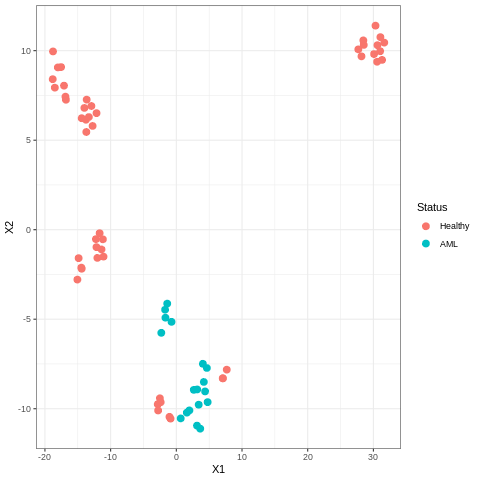
\includegraphics[width=.5\textwidth]{figs/tsnep10.png}\hfill
        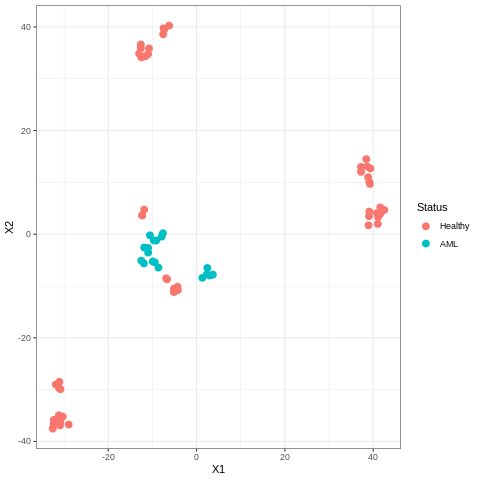
\includegraphics[width=.5\textwidth]{figs/tsnep5.png}\hfill
         \caption{کاهش بعد داده ها به ترتیب با  مقادیر \lr{perplexity} ۵ ۱۰ ۱۵ ۲۰}
	\label{fig:tsnep}
\end{figure}
در نهایت با اندکی تغیر دادن فضای سرچ در پارانتر \lr{prep} بهترین نتیجه با  \lr{prep = 8} 
حاصل می‌شود.
که در شکل 
\ref{fig:prep8}
می‌توانید مشاهده کنید.
\begin{figure}[h!]
	\centering
	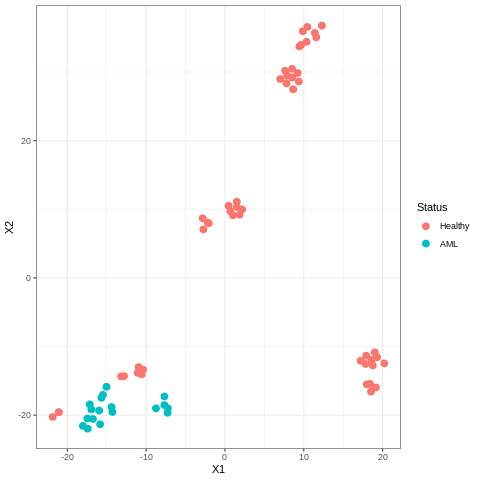
\includegraphics[width=0.5\columnwidth]{figs/prep8.png}
	\caption{کاهش بعد با \lr{prep8=8}}
	\label{fig:prep8}
\end{figure}
\subsection{\lr{MDS}}
این کاهش بعد سعی می‌کند که فاصله نسبی بین داده ها در بعد کمتر حفظ شود.
دقت کنید که در \lr{pca} هدف حفظ واریانس داده ها بود. در اینجا هدف حفظ فاصله نسبی دو به دو داده ها خواهد بود.

برای این کار ما ۳ روش از روش های موجود در \lr{R }
را انجام می‌دهیم.
\subsubsection{\lr{Principal Coordinates Analysis}}
نتایج در شکل \ref{fig:pco}
\begin{figure}[h!]
	\centering
	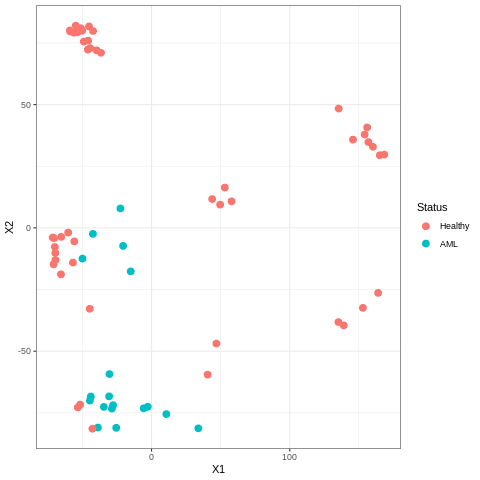
\includegraphics[width=0.5\columnwidth]{figs/pco.png}
	\caption{کاهش بعد با \lr{pco}}
	\label{fig:pco}
\end{figure}
\subsubsection{\lr{Stress Minimization: SMACOF}}
نتایج در شکل \ref{fig:mds}
\begin{figure}[h!]
	\centering
	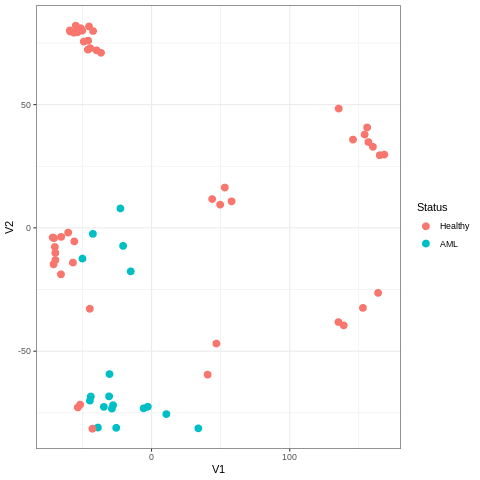
\includegraphics[width=0.5\columnwidth]{figs/mds.png}
	\caption{کاهش بعد با \lr{SMACOF}}
	\label{fig:mds}
\end{figure}
\subsubsection{\lr{Sammon}}
نتایج در شکل  \ref{fig:sammon}
\begin{figure}[h!]
	\centering
	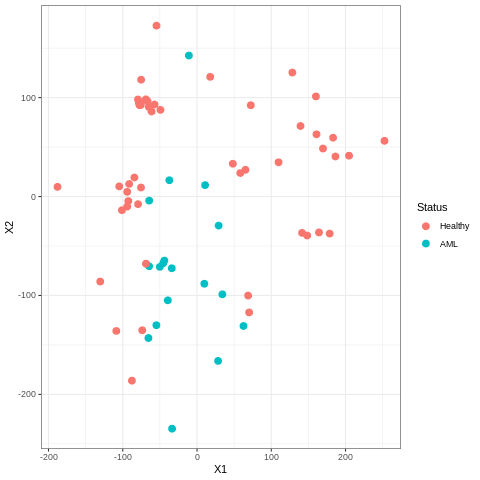
\includegraphics[width=0.5\columnwidth]{figs/sammon.png}
	\caption{کاهش بعد با \lr{sammon}}
	\label{fig:sammon}
\end{figure}
\subsection{انتخاب بهترین کاهش بعد}
از آنجا که هدف ما کاهش بعد داده ها به صورتی است که تفاوت معناداری بین سمپل های بیمار و سالم حاصل شود.
در واقع اگر بخواهیم یک مدل لرنینگ یا هر معیار تصمیم گیری دیگری قرار دهیم تا بتواند به ما کمک کند بهتر است که تفاوت یا \lr{margin} بین داده ها بیشتر شود که در حالت \lr{TSNE with prep = 5}  از بقیه کاهش بعد ها بهتر عمل می‌کند.
زیرا هم داده ها تفاوت معنا داری دارند.
هم داده های \lr{AML}
در این حالت رفتار یک توزیع پارامتری دارند.

\section{همبستگی بین گروه‌ها}
هرکدام از انواع \lr{Source Name} در واقع نشان‌دهنده نوع خاصی از سلول‌ها را نشان می‌دهد که از نمونه مورد نظر گرفته شده است.

نمودار هم‌بستگی بین گروه‌های مختلف در شکل \ref{fig:sourcename-cor-heatmap} رسم شده است.
با توجه به نمودار هم‌بستگی، گروه \lr{Granulocytes} هم‌بستگی نسبتا پایینی با گروه نمونه‌های بیمار دارد. 
و از طرفی نمونه‌های \lr{T Cells} و \lr{B Cells} هم‌بستگی قابل توجهی با نمونه‌های بیمار دارند.

لزوم انجام این مرحله شناسایی گروهی از نمونه‌های سالم است که شباهت بیشتری با گروه بیمار دارند.
شناسایی بیماران از این گروه نمونه‌های سالم و بررسی آن‌ها ما را به نتایج ارزشمندتری می‌رساند (زیرا گروه دیگر نمونه‌های سالم تفاوت فاحشی با گروه بیمار دارند که تصمیم‌گیری براساس آن‌ها لزوما نتیجه خوبی نخواهد داشت).
هم‌چنین می‌دانیم که هر‌چه سلول‌ها در هر گروه به هم شبیه‌تر باشند، تحلیل بهتر خواهد بود.

\begin{figure}[h!]
	\centering
	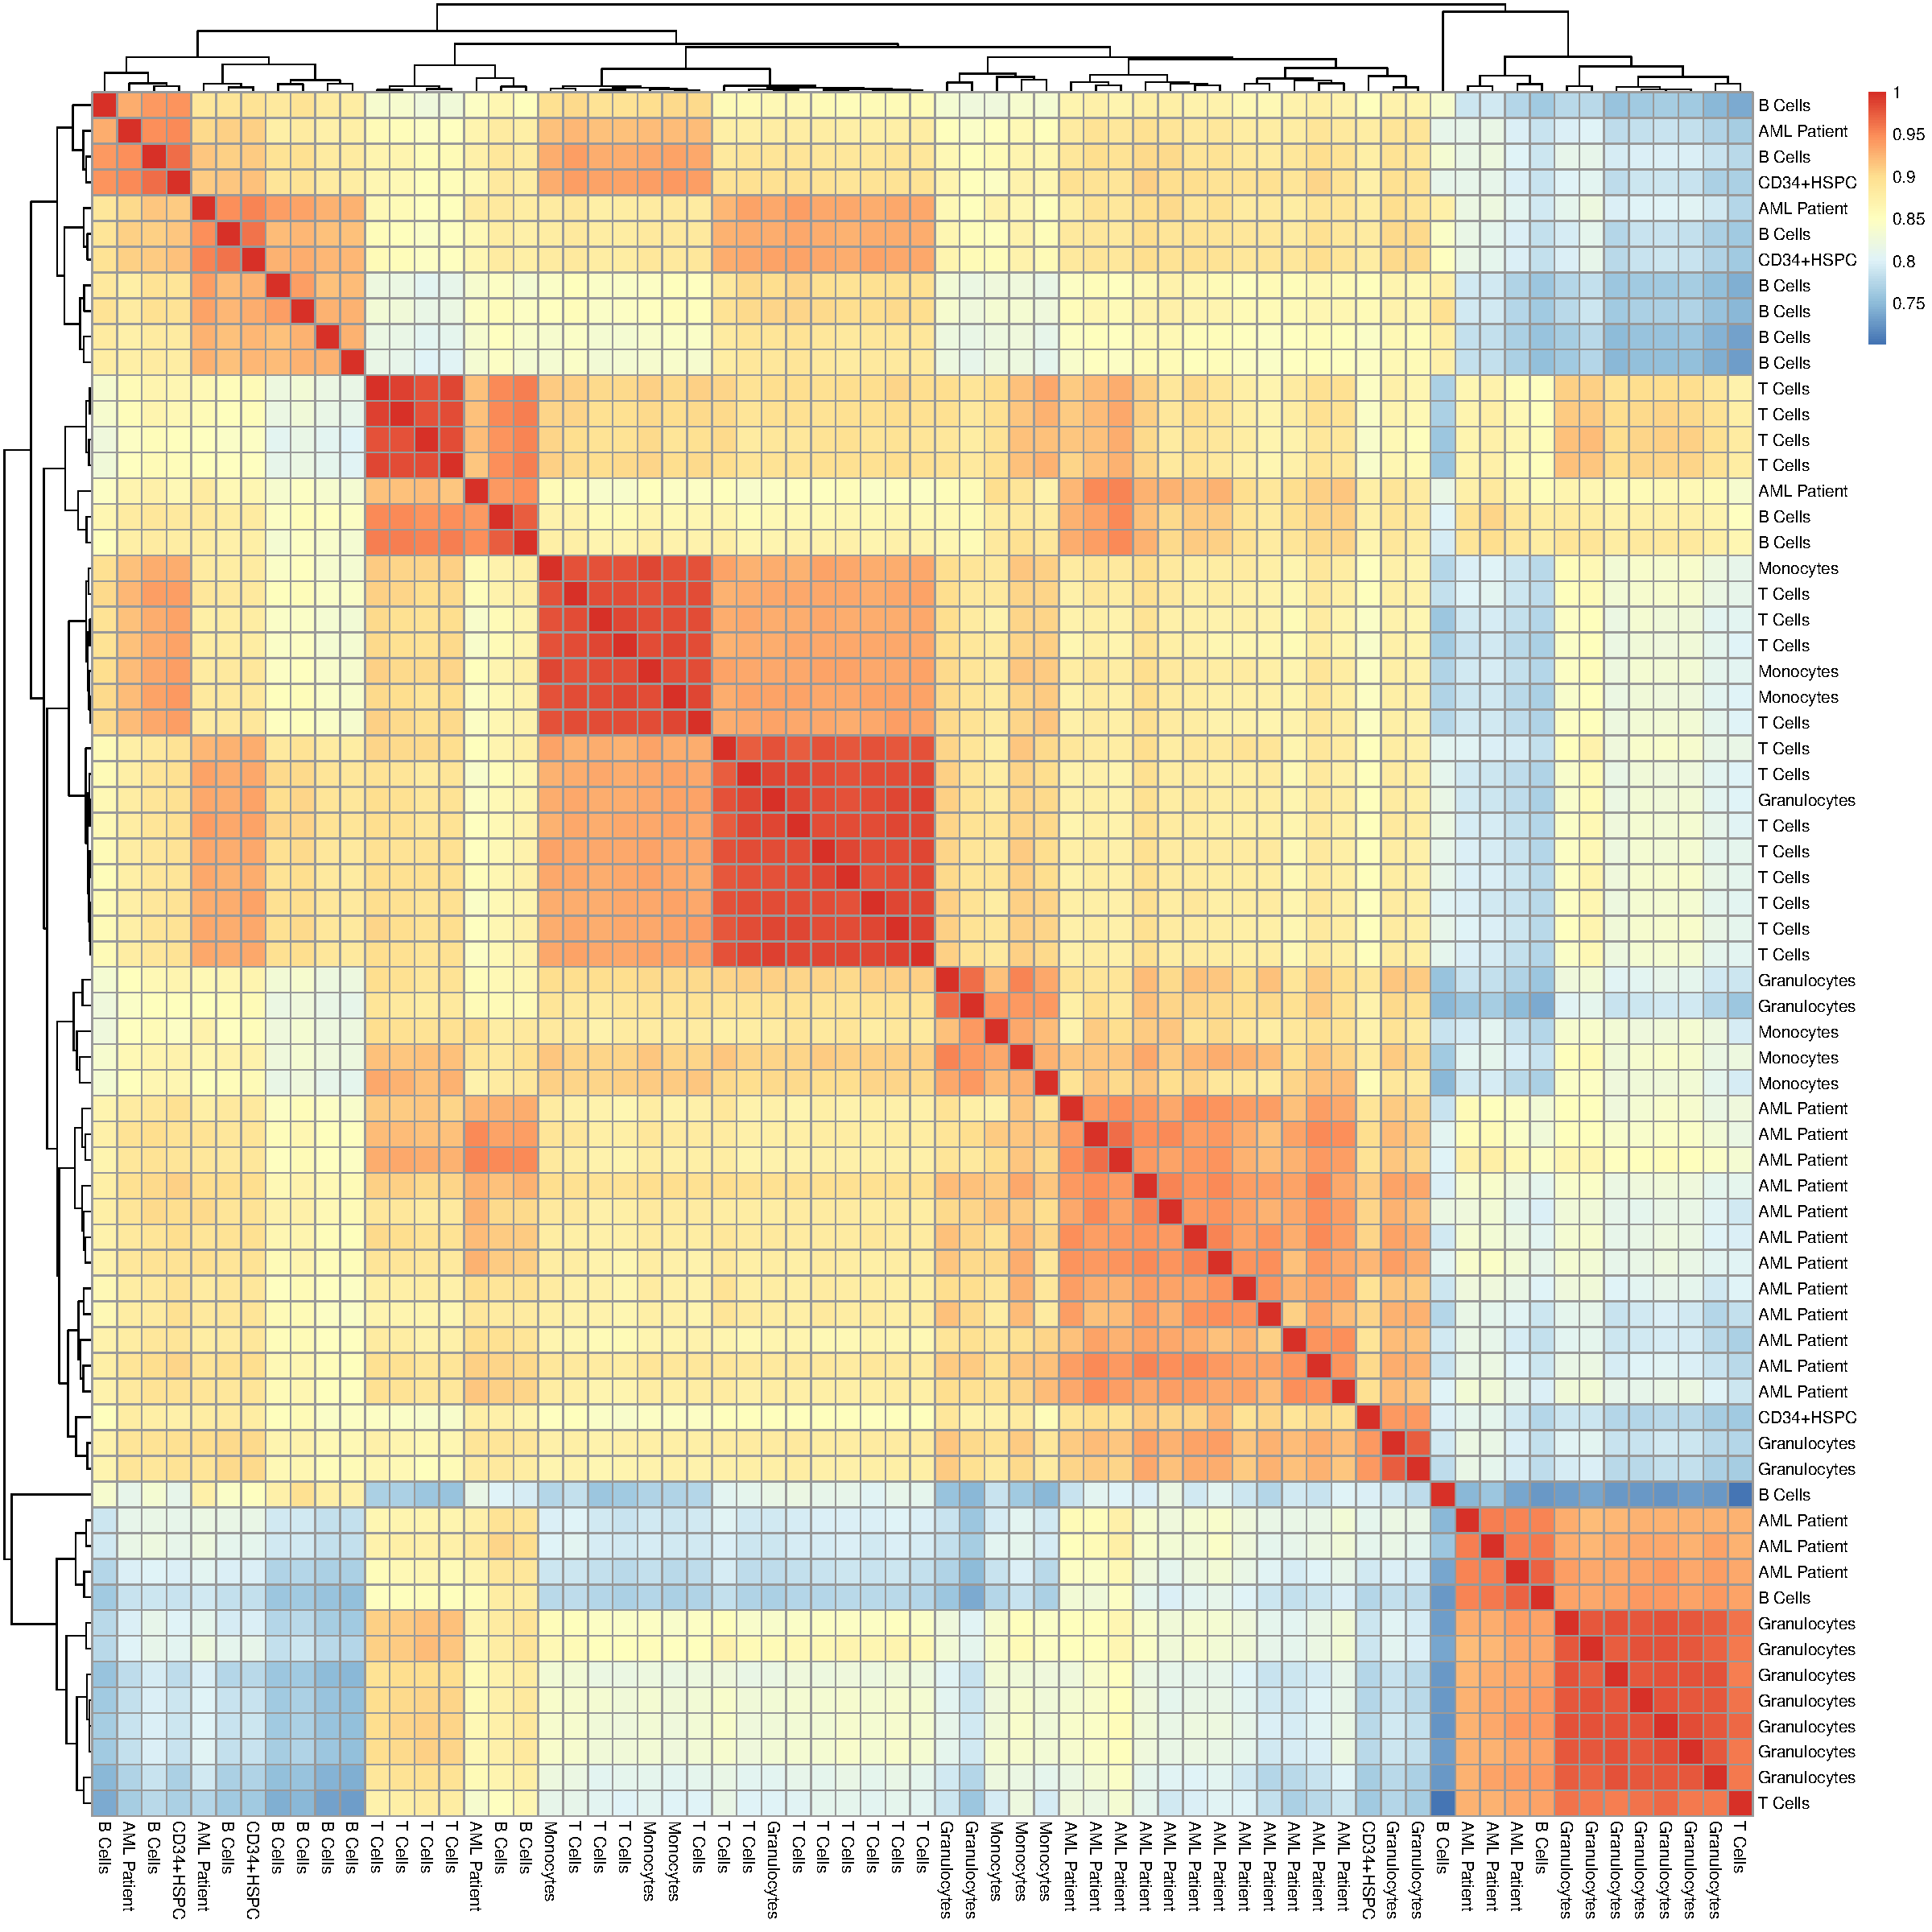
\includegraphics[width=0.8\columnwidth]{figs/SourceName-Cor-Heatmap.pdf}
	\caption{میزان هم‌بستگی نمونه‌ها با یک‌دیگر}
	\label{fig:sourcename-cor-heatmap}
\end{figure}


\clearpage

\begin{thebibliography}{99}
	\begin{latin}
		\bibitem{nature-microarray}
		Nature Defenition Microarray (2014), Nature Education, \url{https://www.nature.com/scitable/definition/microarray-202}
		
		\bibitem{wiki-microarray}
		Microarray Hitmap (2006), Wikipedia, \url{https://commons.wikimedia.org/wiki/File:Heatmap.png#/media/File:Heatmap.png}
		
		\bibitem{geo-data}
		GEO study, R tidyverse, \url{https://lsru.github.io/tv_course/TD_project_solution.html}
		
%		\bibitem{lamport94}
%		Leslie Lamport (1994) \emph{\LaTeX: a document preparation system}, Addison
%		Wesley, Massachusetts, 2nd ed.
	\end{latin}
\end{thebibliography}



\end{document}
